\begin{frame}{Two Primary Questions}
  \onslide<+->{Previous work focused on two primary questions.  These form the basis of this work.}
  \vfill
    \begin{itemize}[<+->]
      \setlength\itemsep{15pt}
      \item How can we produce \textit{strong} adversarial examples that fool the model with high confidence while requiring only a small perturbation?

      \item How can we train a model so there are no \only<+->{(\textit{easily found})} adversarial examples?
    \end{itemize}
  \vfill
  \onslide<+->{We will tackle these two questions separately with the first one being much more interesting}
\end{frame}

\section{Producing Strong Adversarial Examples}
\transitionFrame{Producing Strong Adversarial Examples}

\begin{frame}{Adversarial Examples should be Intractable}

  \onslide<+->{\textbf{\green{Inner Maximization}}: Adversarial example generation problem:
      \begin{equation}\label{eq:InnerMaximization}
        \max_{\delta \in \sPerturb} \loss (\X + \perturb, \y ; \params)
      \end{equation}

    \vspace{-3pt}
    is a highly non-concave function.  Potentially large number of local maxima making this problem \textit{seem} intractable.
  }

  \vfill
  \begin{itemize}[<+->]
    \setlength{\itemsep}{8pt}
    \item \textbf{\red{Previous Work}}: Fast Gradient Sign Method (FGSM)
    \item \textbf{\blue{\madry's Solution}}: Projected Gradient Descent (PGD)
  \end{itemize}
\end{frame}


\begin{frame}{Previous Work: Fast Gradient Sign Method}
  \onslide<+->{%
    \begin{definition}
      \textbf{\blue{Fast Gradient Sign Method}} (FGSM) linearizes the inner maximization s.t.:

      \begin{equation}\label{eq:FGSM}
        \xadv = \X + \varepsilon \sgn\left(\nabla_{\X} \loss(\X, \y ; \params) \right)
      \end{equation}
    \end{definition}
  }

  \begin{itemize}[<+->]
    \setlength\itemsep{8pt}
    \item \textbf{Summary}: Simple ``single-step-size'' approach
    \item Enhanced versions of FGSM (e.g., multi-step, randomized) that are beyond the scope of this talk
  \end{itemize}

  \vspace{3pt}
  \onslide<+->{\textbf{\red{Major Issue}}: FGSM provides no security guarantee}
  \begin{itemize}[<+->]
    \setlength\itemsep{8pt}
    \item \textbf{Why?} \onslide<+->{Not selecting the \textit{worst-case} perturbation}
    \item Easy to find ``nearby'' perturbations with significantly higher loss
  \end{itemize}
\end{frame}


\begin{frame}{Projected Gradient Descent}
  \onslide<+->{A type of \green{\textit{constrained optimization}} with the constraint is a \blue{\textit{projection}}}

  \vfill
  \onslide<+->{
    \begin{definition}
      A \textbf{\blue{projection}} of a point~$z$ onto a set~$\mathcal{X}$ is defined as:

      \[ \Pi_{\mathcal{X}}(z) = \argmin_{\X \in \mathcal{X}} \norm{\X-z}^{p}\text{.}  \]
    \end{definition}
  }

  \vfill
  \begin{itemize}[<+->]
    \item $\Pi_{X}$ is the projection operator
  \end{itemize}
\end{frame}


\begin{frame}{Projected Gradient Descent --- The Algorithm}
  \begin{columns}
    \begin{column}{0.5\textwidth}
      \textbf{Procedure}:
      \begin{enumerate}[<+->]
        \setlength{\itemsep}{12pt}
        \item For any ${\X \in \mathcal{X}}$, define ${\X^{(0)} = \X + \delta}$ where ${\perturb \sim \mathcal{U}\left( \sPerturb \right)}$
        \item For each time $t$, define:
          \begin{equation}\label{eq:PGD:GradUpdate}
            z^{(t+1)} = \X^{(t)} \textcolor<+->{red}{-} \alpha \nabla_{\X} \loss(\X^{(t+1)}, \y_{\X}) \text{.}
          \end{equation}
        \item Enforce the constraint where:
          \begin{equation}\label{eq:PGD:NextX}
            \X^{(t+1)} = \Pi_{\mathcal{\mathcal{X}}}(z^{(k+1)}) \text{.}
          \end{equation}

        \item Repeat steps~\#2 and~\#3 until convergence
      \end{enumerate}
    \end{column}
    \begin{column}{0.45\textwidth}
      \begin{center}
        \onslide<+->{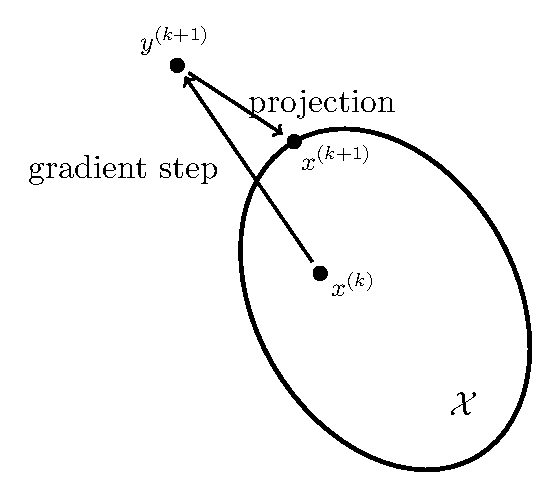
\includegraphics[scale=0.65]{pgd}~\cite{Srebro}}
      \end{center}
    \end{column}
  \end{columns}
\end{frame}

\subsection{\texorpdfstring{$\ell_{p}$}{Lp} Balls}
\transitionFrame{To go further, we need to understand $\ell_{p}$ balls\ldots}

\begin{frame}{$\ell_{p}$ Balls --- Norms First}
  For ${x \in \mathbb{d}}$, the $L_{p}$ norm is:

  \begin{equation}\label{eq:LpNorm}
    \norm{x}_{p} = \left( \sum_{i=1} x_{i}^{p}  \right)^{\frac{1}{p}}
  \end{equation}

  $L_{\infty}$ norm is a special a case:

  \begin{equation}\label{eq:LinftyNorm}
    \norm{x}_{\infty} = \sup_{i} \abs{x_i}
  \end{equation}

  \begin{center}
    \textbf{Note}: $\sup$ equals the $\max$ for a finite set
  \end{center}
\end{frame}

\begin{frame}{$\ell_{p}$ Balls --- Formally}
  \begin{definition}
    Given scalar ${\varepsilon > 0}$, the $\ell_{p}$~ball of a point ${x \in \mathbb{R}^{d}}$ is:

    \begin{equation}\label{eq:LpBall}
      \ell_{p}(x) = \setbuild{x + \delta}{\norm{\delta}_{p} \leq \varepsilon}\text{.}
    \end{equation}
  \end{definition}

  \begin{columns}
    \begin{column}{0.5\textwidth}
      \onslide<2->{Let's visualize $\ell_{p}$ for different values of $p$}

      \vspace{15pt}
      \onslide<4->{\blue{\textbf{Question}}: What is the value of $\varepsilon$?}

      \vspace{4pt}
      \onslide<5->{\textbf{Answer}: $\varepsilon = 1$}

      \vspace{15pt}
      \onslide<6->{\green{\textbf{Key Takeaway}}: $\ell_{\infty}$~ball is a superset of all other $\ell_{p}$~balls for fixed $\varepsilon$}
    \end{column}
    \begin{column}{0.45\textwidth}
      \onslide<3->{
        \begin{center}
          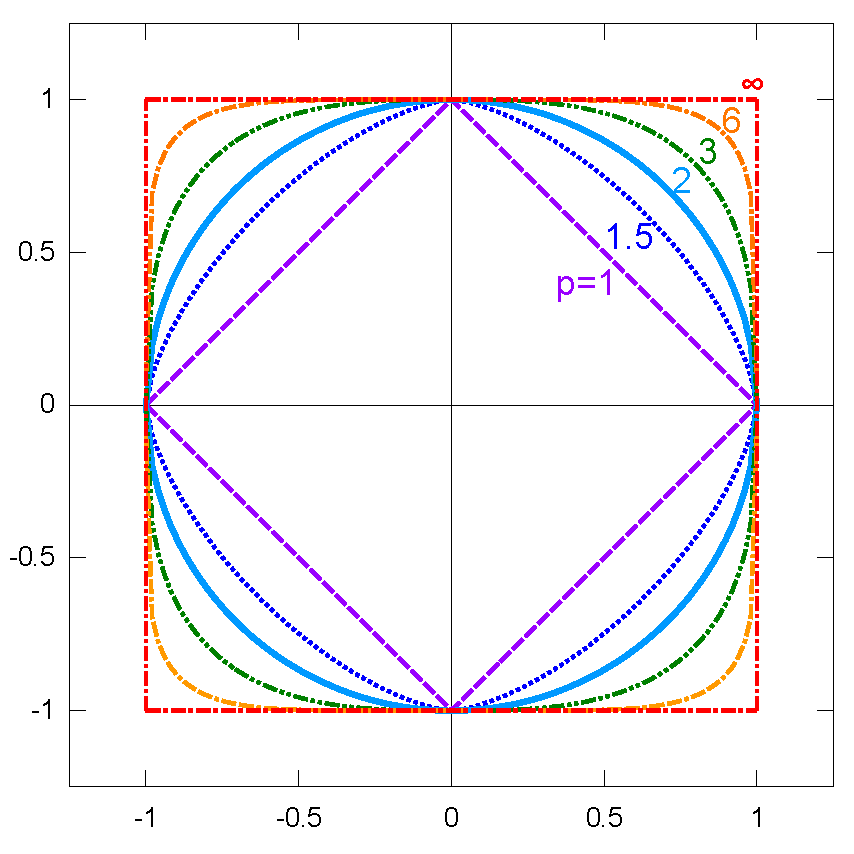
\includegraphics[scale=0.28]{img/lpballs.pdf}~\cite{wiki:Lp_space}
        \end{center}
      }
    \end{column}
  \end{columns}
\end{frame}


\subsection{\texorpdfstring{$\ell_{\infty}$}{L-infinity}~Ball \& PGD}

\begin{frame}{Connecting $\ell_{\infty}$ \& PGD}

\end{frame}

\begin{frame}{PGD \& Adversarial Tractability}
  \onslide<+->{\textbf{\blue{Question}}: Does PGD + $\ell_{\infty}$~balls guarantee eliminate \textit{all} adversarial examples within (Minkowski) distance~$\varepsilon$ of $\X$?}

  \vspace{3pt}
  \onslide<3->{\textbf{Answer}: No.} \only<4-5>{Why?}
  \begin{itemize}
    \item \onslide<5->{PGD is only a \textbf{first-order adversary}.}
  \end{itemize}

  \vfill
  \onslide<6->{
    \begin{definition}
      \blue{\textbf{First-order Adversary}} is the strongest attack utilizing only \textit{first-order} (e.g.,~gradient) information about network
    \end{definition}
  }

  \vfill
  \onslide<7->{An attacker using higher order information (e.g.,~Hessian) may tractably find adversarial examples.}
  \begin{itemize}
    \item \onslide<8->{Similar to a \textit{polynomially-bounded} adversary that is the cornerstone of cryptography}
  \end{itemize}
\end{frame}

\subsection{Zero-Order Adversaries}
\begin{frame}{Zero-Order Adversaries}
  \begin{itemize}[<+->]
    \setlength{\itemsep}{20pt}
    \item A \blue{\textbf{zero-order adversary}} has no direct access to the classifier and is only able to evaluate the classifier based on chosen examples
      \begin{itemize}
        \item ``Zero-order'' means no access to ``first-order'' information
        \item \textit{Translation}: \red{No gradient feedback}
      \end{itemize}

    \item \textit{Example}: Black-box attacker

    \item Much more challenging that one-day attacker
  \end{itemize}
\end{frame}
